\documentclass{standalone}
\usepackage{tikz}

\usetikzlibrary{calc,math}


\newcommand{\TRIANGLE}[4]{
  \draw #1 -- #2 -- #3 -- cycle;
  \node[font=\tiny] at ($ #1 ! 0.5 ! #2 ! 0.333 ! #3 $) { #4 };
}

\begin{document}

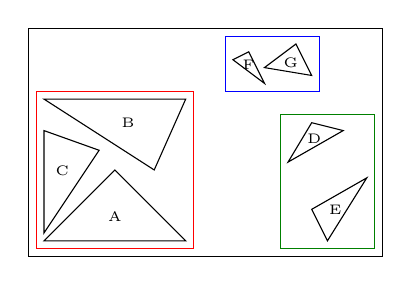
\begin{tikzpicture}
  \TRIANGLE{(0.1,0.1)}{(1.9,0.1)}{(1, 1)}{A}
  \TRIANGLE{(1.9,1.9)}{(1.5,1)}{(0.1, 1.9)}{B}
  \TRIANGLE{(0.1,0.2)}{(0.8,1.25)}{(0.1, 1.5)}{C}
  \draw[red] (0,0) rectangle (2,2);

  \TRIANGLE{(3.2,1.1)}{(3.9,1.5)}{(3.5,1.6)}{D}
  \TRIANGLE{(3.5,0.5)}{(3.7,0.1)}{(4.2,0.9)}{E}
  \draw[green!50!black] (3.1,0) rectangle (4.3,1.7);

  \TRIANGLE{(2.5,2.4)}{(2.9,2.1)}{(2.7,2.5)}{F}
  \TRIANGLE{(2.9,2.3)}{(3.5,2.2)}{(3.3,2.6)}{G}
  \draw[blue] (2.4,2.0) rectangle (3.6,2.7);

  \draw (-0.1,-0.1) rectangle (4.4,2.8);
\end{tikzpicture}

\end{document}
